\section{Overview of Machine Learning Algorithms}
\subsection{Neural network}
Neural networks were first introduced in 1944 by two University of Chicago researchers Warren McCullough and Walter Pitts, who later moved to MIT in 1952. These algorithms are modeled loosely after the human brain, that are designed to recognize patterns.  Dr. Robert Hecht-Nielsen, inventor of the first neurocomputer defines a neural network as:
"...a computing system made up of a number of simple, highly interconnected processing elements, which process information by their dynamic state response to external inputs"\cite{Caudill}.
\begin{figure}[htb!]
    \centering
    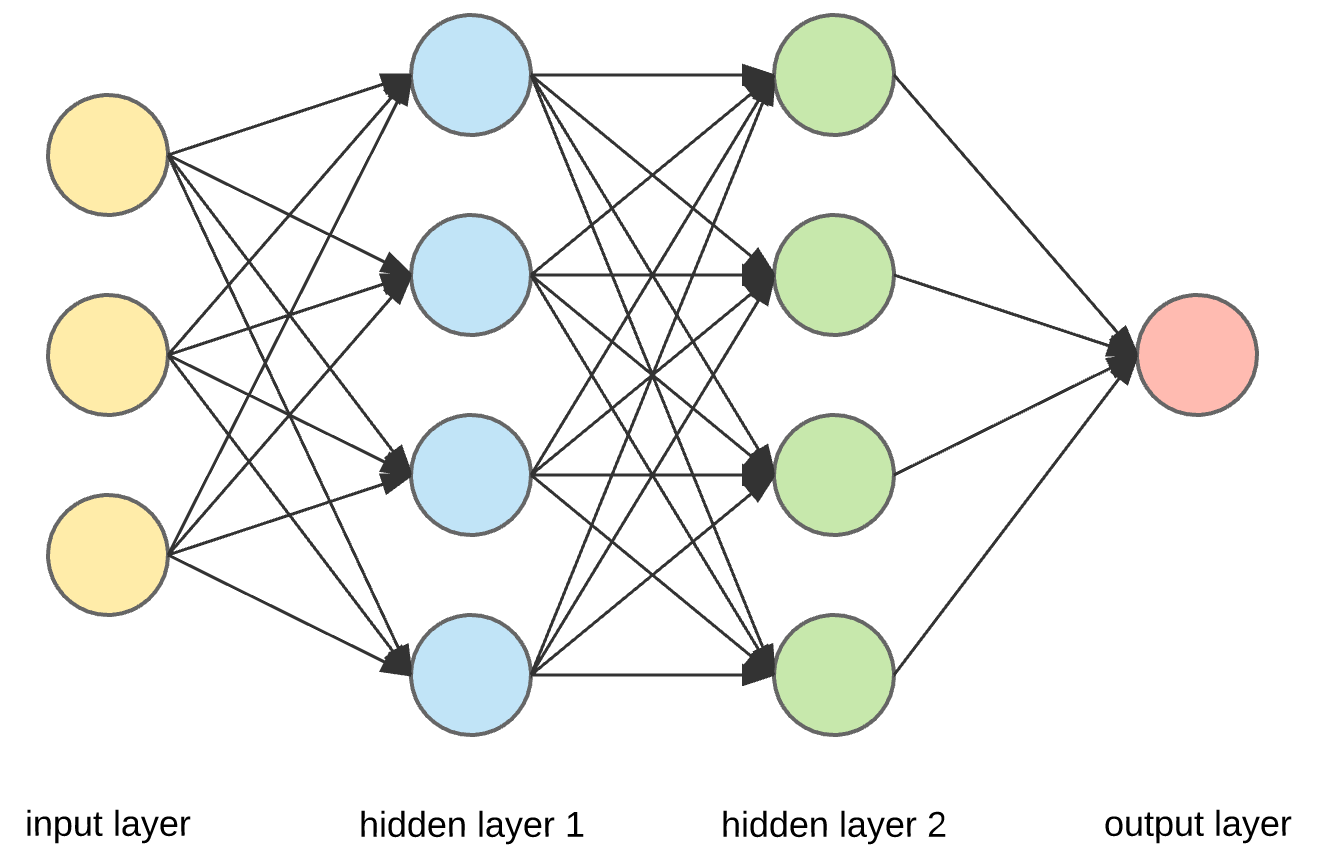
\includegraphics[scale=0.15]{files/nn.png}
    \caption{Neural network}
    \label{Neural network}
    \end{figure}
    \FloatBarrier
% cite figure: https://towardsdatascience.com/applied-deep-learning-part-1-artificial-neural-networks-d7834f67a4f6
A typical neural network looks like a variation of Figure 2.1. \\
Input layer: The leftmost layer in the network is made up of input neurons and the layer is called the input layer. There is no computation performed in the nodes at this layer. Input layer simply provides the information from the environment to the next layer.
Hidden layers: The layers in the middle make up the hidden layers, as the neurons in these layers are neither inputs nor outputs. There can be zero or multiple hidden layers. Hidden layers takes the input from the input layer and passes information to the output layer after performing computation on the data. 
Output layer: The rightmost or output layer contains the output neurons, or, as in this case, a single output neuron. 
There are no set rules to design the layers of a neural network (specially the hidden layers) and this process is often considered as an art\cite{NN}. We determine the number of hidden layers and nodes empirically for each particular case in order to optimize performance. The edges (or connections) between a layer and the layer before it are represented by a weight $\omega_{ij}$, which represents the strength of connection between i and j nodes. During the training phase of the neural network, we assign random values to the weights for each connection. The algorithm then tries to optimize the weights so that the error function is minimized. For each node at a layer all the output from the previous node is multiplied by the weight of connections between them and the sum of all the different connections produces the value at that node. This cycle is repeated for all the nodes in every layer. The algorithm compares the prediction from the output layer to the real value and readjusts the weights. Once the optimal value is reached the network can be used to make predictions\cite{hall199}.

These neural networks where the output from one layer is used as input to the next layer are called feedforward neural networks\cite{NN}\cite{hall199}. There are no loops in the feedforward neural network and the information flows in one direction and are never fed back. The most well known form of a feed forward neural network is called multilayer perceptron(MLP). MLPs are also called universal function approximator. A single hidden layer MLP with a sufficient number of nonlinear units can act as a continuous function on to a narrow input domain with arbitrary precision. \cite{Graves}.
There are some other models of artificial neural networks in which feedback loops are possible. These models are called recurrent neural networks. The idea in these models is to have neurons which fire for some limited duration of time, before becoming quiescent. That firing can stimulate other neurons, which may fire a little while later, also for a limited duration. That causes still more neurons to fire, and so over time we get a cascade of neurons firing. Loops don't cause problems in such a model, since a neuron's output only affects its input at some later time, not instantaneously. Recurrent neural nets have been less influential than feedforward networks, in part because the learning algorithms for recurrent nets are (at least to date) less powerful. But recurrent networks are still extremely interesting. They're much closer in spirit to how our brains work than feedforward networks. And it's possible that recurrent networks can solve important problems which can only be solved with great difficulty by feedforward networks.\cite{NN} % cite: http://neuralnetworksanddeeplearning.com/chap1.html



\subsection{Convolutional neural network}
Convolutional neural networks (ConvNet) are very similar to ordinary neural networks in structure. They work by extracting simple features at a higher resolution and then converting them into more complex features at a coarser resolution \cite{simard2003best}. It does so by performing dot product on the inputs received at each neuron and optionally follow it with non-linearity. Just like a normal neural network, convolutional neural network (from the input image to output class) can be expressed as a single differential function. It also has a loss function on the fully-connected output layer.

Convolutional Neural Networks (ConvNet) are very similar to ordinary Neural Networks. they are made up of neurons that have learnable weights and biases. Each neuron receives some inputs, performs a dot product and optionally follows it with a non-linearity. The whole network still expresses a single differentiable score function: from the raw image pixels on one end to class scores at the other. And they still have a loss function (e.g. SVM/Softmax) on the last (fully-connected) layer and all the tips/tricks we developed for learning regular Neural Networks still apply. 
What makes it different is that ConvNet architectures make the explicit assumption that the inputs are images, which allows us to encode certain properties into the architecture. These then make the forward function more efficient to implement and vastly reduce the amount of parameters in the network. Convolutional Neural Networks take advantage of the fact that the input consists of images and they constrain the architecture in a more sensible way. In particular, unlike a regular Neural Network, the layers of a ConvNet have neurons arranged in 3 dimensions: width, height, depth. (Note that the word depth here refers to the third dimension of an activation volume, not to the depth of a full Neural Network, which can refer to the total number of layers in a network). 
A ConvNet architecture is made up of the following layers: \\
Input: This layer holds the raw input image in form of it's pixel values and color channels.\\
Convolutional layer: This layer computes the dot product between it's weight and a small region in the previous layer it is connected to.\\
Rectified linear unit: \\
Fully connected layer: The fully connected output layer computes the class scores for the input. The neurons in this layer are connected to every neuron in the last layer.\\

A simple ConvNet is a sequence of layers, and every layer of a ConvNet transforms one volume of activations to another through a differentiable function. We use three main types of layers to build ConvNet architectures: Convolutional Layer, Pooling Layer, and Fully-Connected Layer (exactly as seen in regular Neural Networks). We will stack these layers to form a full ConvNet architecture.


RELU layer will apply an elementwise activation function, such as the $max(0,x)$ thresholding at zero. This leaves the size of the volume unchanged ([32x32x12]).
POOL layer will perform a downsampling operation along the spatial dimensions (width, height), resulting in volume such as [16x16x12].
FC (i.e. fully-connected) layer will compute the class scores, resulting in volume of size [1x1x10], where each of the 10 numbers correspond to a class score, such as among the 10 categories of CIFAR-10. As with ordinary Neural Networks and as the name implies, each neuron in this layer will be connected to all the numbers in the previous volume.
\begin{figure}[htb!]
    \centering
    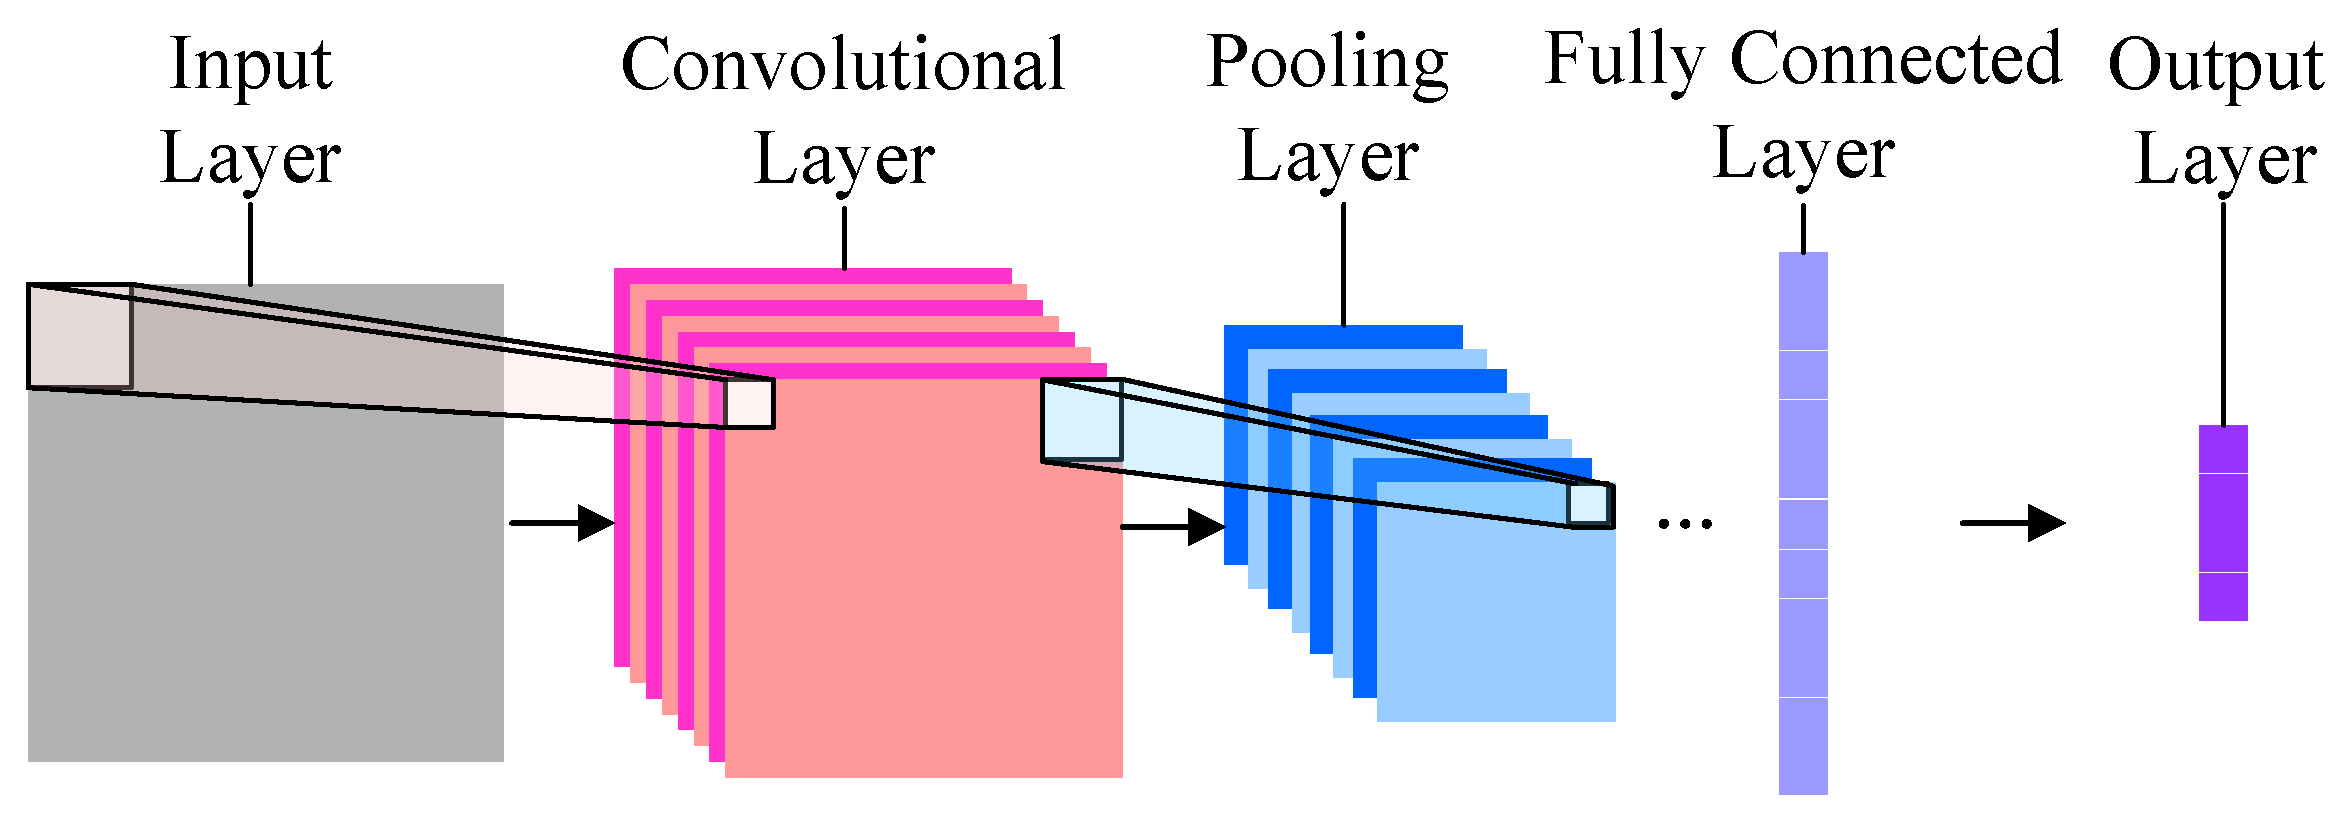
\includegraphics[scale=1.25]{chapters/litReview/files/convNet.png}
    \caption{Convolutional Neural network \cite{convNN}}
    \label{Neural network}
    \end{figure}
    \FloatBarrier

Note that some layers contain parameters and other don’t. In particular, the CONV/FC layers perform transformations that are a function of not only the activations in the input volume, but also of the parameters (the weights and biases of the neurons). On the other hand, the RELU/POOL layers will implement a fixed function. The parameters in the CONV/FC layers will be trained with gradient descent so that the class scores that the ConvNet computes are consistent with the labels in the training set for each image.
%cite http://cs231n.github.io/convolutional-networks/

\subsection{Naive Bayes}
In it's simplest form a Naive Bayes algorithm is a type of Bayesian network where all attributes are independent given the value of the class variable. This property is called conditional independence. It is obvious that the conditional independence assumption is rarely true in most real-world applications\cite{zhang2004optimality}. Despite this limitation the algorithm is very popular and works quite well in many real-world situations like document classification and spam filtering. The classifier is a really common supervised learning algorithm because it is fast, easy to implement and relatively effective. They also require relatively small number of training data to estimate the necessary parameters of the network\cite{scikit-learn}. Given a class variable $y$ and dependent feature vector $x_{1}$...$x_{n}$, Bayes theorem states that:
\begin{center}
    $P(y|x_{1},...,x_{n}) = \frac{P(y)P(x_{1},...,x_{n}|y)}{P(x_{1},...,x_{n})}$
\end{center}
From the conditional independence of features, and, value of a class we know that: 
\begin{center}
$P(y \mid x_1, \dots, x_n) = \frac{P(y) \prod_{i=1}^{n} P(x_i \mid y)}
                                 {P(x_1, \dots, x_n)}$
\end{center}
% Include the equations from https://scikit-learn.org/stable/modules/naive_bayes.html
For a given input $P(x_{1},...,x_{n})$ is constant. Therefore 
\begin{center}
$P(y \mid x_1, \dots, x_n) \propto P(y) \prod_{i=1}^{n} P(x_i \mid y)$
\end{center}
And an expected classification $\hat{y}$ can be obtained by:
\begin{center}
$\hat{y} = \arg\max_y P(y) \prod_{i=1}^{n} P(x_i \mid y)$
\end{center}
The main distinction between different versions of naive Bayes classifiers are the assumptions they make about the distribution of $P(x_i \mid y)$\cite{scikit-learn}. The multinomial Naive Bayes suffers from a systematic problem of assigning poor weights to necessary parameters if once class has more training examples than others. This effect lowers the weights for classes with less training examples\cite{rennie2003tackling}. For this reason we have equal numbers of training and testing examples for each class in our experiment. 

\subsection{k-Nearest Neighbor}
The nearest neighbor classifier is a supervised classification technique which assigns an input sample vector (whose classification is to be predicted) to the class of it's nearest neighbors. The similarity between the input and the neighbors is calculated based on some distance metrics. This process does not require any pre-processing of the labeled set of neighbors before their use \cite{cover1967}. This idea can be further extended to assign the class of input variable to the class represented by majority of the $k$ nearest neighbors, where $k$ is a positive number specified by the user. The optimal value of $k$ depends on the data. A larger value of $k$ makes the classification boundaries less distinct while suppressing the noise effect \cite{scikit-learn}. One problem with implementing $k$ nearest algorithm is that in some cases there may be a tie among classes between the $k$ neighbors. This problem can be solved by restricting the values of $k$. In a binary classification problem, the values of $k$ can be restricted to odd numbers so that ties can be avoided. In a multi-class classification, this can be resolved by assigning the input to the class for which the sum of distance to each neighbor is the least. This could further lead to a tie and in that case an arbitrary assignment can be made \cite{keller1985}.
\begin{figure}[htb!]
    \centering
    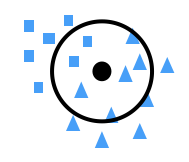
\includegraphics[scale=1]{files/knn.png}
    \caption{$k$-Nearest neighbor}
    \label{k-Nearest neighbor}
    \end{figure}
    \FloatBarrier

\cite{cover1967}
A set of n pairs is given $(x1,\theta 2),...(xn,\theta n)$ s.t the x′is take value in a metric space X upon which is defined a metric d.
The category $\theta$ i is assigned to the ith sample or individual from finite subset {1,2, ... M} and xi is the measurement made upon that ith.
we shall say ”xi belongs to $\theta$ i” when we mean precisely that the ith sample have measurement xi with category $\theta i$ .
Our Goal is to classify the measurement x , for a new arriving pair $(x,\theta )$, the classification is procedure to estimate the $\theta$  since x is observable .
The estimation of $\theta$  is done by utilizing the fact that we have set of n correctly classified points.
We shall call : nearest neighbor of x if
'xn ∈(x1,x2,x3,....xn)'
min d(xi,x) = d(xn,x) i = 1,2,3...,n.

In this case the decision of the nearest neighbor rule is assigning the category $\theta$ n to our new measurement x .
The 1-NN rule decide x belongs to the category of nearest neighbor and ignored the others!.
In general k-NN rule decide x belongs to the category of majority vote of the nearest k neighbors.



\subsection{Support vector machine}
A support vector machine (SVM)  is a supervised machine learning classifier. The support vectors lie on the dotted hyperplanes parallel to the separating hyperplane. The margin, the minimum gap between the supporting hyperplane and the separating hyperplane, is chosen to be maximum. The pseudo-code is a common, abstract description of implemented SMO computer programs. Because SMO is an algorithm for solving the SVM optimization problem, it corresponds to the model constructor and is an abstract version of the quasi-testable core.\cite{Nakajima2016}


support vector machines (SVMs), based on statistical learning theory, are gaining applications in the areas of machine learning, computer vision and pattern recognition because of high accuracy and good generalisation capability

Based on the structural risk minimization (SRM) principal, SVM can get decision-making rules and achieve small error for independent tests set and hence can solve the learning problems efficiently \cite{svm2008}. Recently SVM is applied to solve the problems such as nonlinear, local minimum and high dimension. In many practical applications, SVM can ensure higher accuracy for a long-term prediction compared to other computational approaches.
SVM is based on the concept of decision planes that define decision boundaries. SVM creates a hyperplane by using a linear model to implement nonlinear class boundaries through some nonlinear mapping input vectors into a high-dimensional feature space \cite{SAMANTA2003657} 

It aims to create a decision boundary between two classes that enables the prediction of labels from one or more feature vectors (6). This decision boundary, known as the hyperplane, is orientated in such a way that it is as far as possible from the closest data points from each of the classes. These closest points are called support vectors.
The most obvious drawback to the SVM algo- rithm, as described thus far, is that it apparently only handles binary classification problems. 
Generalizing to multiclass clas- sification is straightforward and can be accom- plished by using any of a variety of methods. To recognize three classes, A, B and C, we simply have to train three separate SVMs to answer the binary questions, “Is it A?,” “Is it B?” and “Is it C?”. More sophisti- cated approaches also exist, which generalize the SVM optimization algorithm to account for multiple classes. \cite{noble2006support}
The SVM algorithm was originally proposed to construct a linear classifier in 1963 by Vapnik (7). An alternative use for SVM is the kernel method, which enables us to model higher dimensional, non-linear models (8). In a non-linear problem, a kernel function could be used to add additional dimensions to the raw data and thus make it a linear problem in the resulting higher dimensional space (Figure 2). Briefly, a kernel function could help do certain calculations faster which would otherwise would need computations in high dimensional space.
It is defined as:

K (x, y)=<f(x), f(y)>

Here K is the kernel function, x, y are n dimensional inputs. f is used to map the input from n dimensional to m dimensional space. <x, y> denotes the dot product. With kernel functions, we could calculate the scalar product between two data points in a higher dimensional space without explicitly calculating the mapping from the input space to the higher dimensional space. In many cases, computing the kernel is easy while going to the high dimensional space to compute the inner product of two feature vectors is hard. The feature vector for even simple kernels can blow up in size, and for kernels like the Radial Basis Function (RBF) kernel (KRBF(x, y) = exp (-γ||x - y||2), the corresponding feature vector is infinite dimensional. Yet, computing the kernel is almost trivial.

The choice of kernel function among other factors could greatly affect the performance of an SVM model. However, there is no way to figure out which kernel would do the best for a specific pattern recognition problem. The only way to choose the best kernel is through trials. We can start with a simple SVM and then experiment with a variety of ‘standard’ kernel functions. Depending on the nature of the problem, it is possible that one kernel is better than the other kernels. An optimal kernel function can be selected from a fixed set of kernels in a statistically rigorous fashion by using cross-validation.

\begin{figure}[htb!]
    \centering
    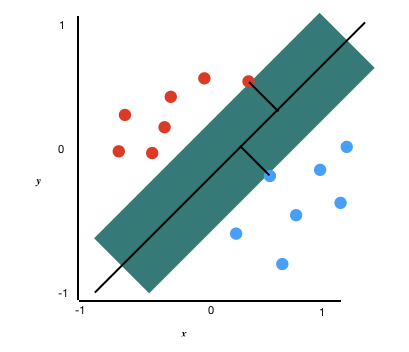
\includegraphics[scale=0.75]{files/svm.png}
    \caption{SVM maximizes the margin between classes}
    \label{SVM maximizes the margin between classes}
    \end{figure}
    \FloatBarrier

